\chapter{Analysis}
\todo{Skrevet om, trengs å leses over}
This chapter provides the background knowledge required to understand the thought process behind the selected technologies.
The group has been researching different technologies and solutions that can be viable for the application we are developing. Throughout the selection process the group have presented the assignment provider, Michael A. Lundsveen with results from the research and recommendations the group has found for the different technologies that can be used for the application. The group together with Michael worked together to select which technologies that should be used based on the this research.

The chapter first inspects the database technologies that are suitable for the assignment.
Afterwards the chapter examines the selected frontend technology before analyzing the technology stack used for the backend development.
Lastly the chapter provides insight as to why the methodology selected is the most suitable for the project.

    

%Ut ifra spørreskjema så skriver vi hva vi fikk ut av det og hva vi lærte av det. Vi har ikke sendt ut spørreskjema enda så denne delen er av den grunn ikke fylt ut.

\todo{Why only looking at the two most popular? Why not others?}
\section{Database technology selection}
The two most popular database systems today are the SQL- and NoSQL-based database systems \cite{stackoverflow-db-statistics}.
The distinction between SQL and NoSQL database systems have become increasingly blurred \cite{sql-vs-nosql}, but there are still key differences between the two which makes them worth analyzing in order to find the most suitable database system for this project.

\iffalse
\subsection{CAP theorem}
The CAP theorem is a theorem within distributed database systems \cite{sql-schema}.
The theorem states that only two out of the following conditions can hold at any time:
\begin{itemize}
    \item Availability.
    This condition states that every request receives a (non-error) response.
    This means the data requested may not necessarily be up-to-date as the node may not have the up-to-date data \cite{sql-schema}.
    \item Consistency.
    This condition states that all nodes have access to the same data.
    This means whenever an attempt to extract data from the database is made the database will either provide up-to-date data or failure \cite{sql-schema}.
    \item Partitioning tolerance.
    This condition states that the database system will continue to operate despite any number of messages between the nodes being delayed or dropped by the network.
    This means the database system can operate normally while sustaining any number of network failures so long as not every node is experiencing failure \cite{sql-schema}.
\end{itemize}

A database is said to support AC when availability and consistency are selected, its said to support AP when availability and partitioning tolerance are selected and its said to support CP when consistency and partitioning tolerance are selected.
\fi

\subsection{SQL} 
SQL(Structured Query Language) is a database language for data management\cite{sql-goal} of a RDBMS(relational database management system) \cite{sql-is-a-rdbms} based on the relational data model proposed by Edgar Frank Todd \cite{rdbms}.
The relational data model logically structures all relations(tables) and each relation is provided a name and is built up of named attributes - columns of data \cite{sql-is-a-rdbms}.
The rows of a table are known as tuples \cite{sql-is-a-rdbms} and, provided the table is normalized for the first normal form or higher, they contain one value per attribute \cite{sql-1nf}.
Figure \ref{fig:relational-db-visualised} illustrates the relational model graphically.

\begin{figure}
    \centering
    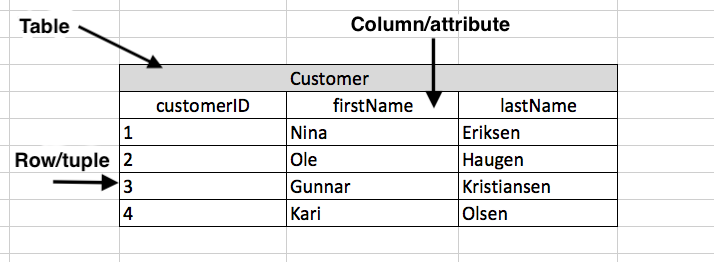
\includegraphics[width=115mm,scale=1]{figures/relational-db-visualised.png}
    \caption{Table named "Customer" containing three attributes and four tuples}
    \label{fig:relational-db-visualised}
\end{figure}

SQL offers a data definition language(DDL) \cite{sql-components}.
The DDL defines the database schema - that is the structure, meaning which attributes the tables consists of, and which tables the database consists of.
It is impossible to add data to the database until a schema has been defined.
The DDL also describes any relational integrities the tables of the database, or the columns of table, may have \cite{sql-constraints}.
In figure \ref{fig:relational-db-relation} a given customer may have several orders but a given order may have one and only one customer associated with it; this is an example of a one-to-many relationship.
In addition to a one-to-many relationship an attribute or table may also have a one-to-one or a many-to-many relationship \cite{sql-relationships}.
Lastly the DDL also defines any security constraints the database may have - such as which users have permissions to read, update or delete the contents of a given table \cite{sql-ddl}.

\begin{figure}
    \centering
    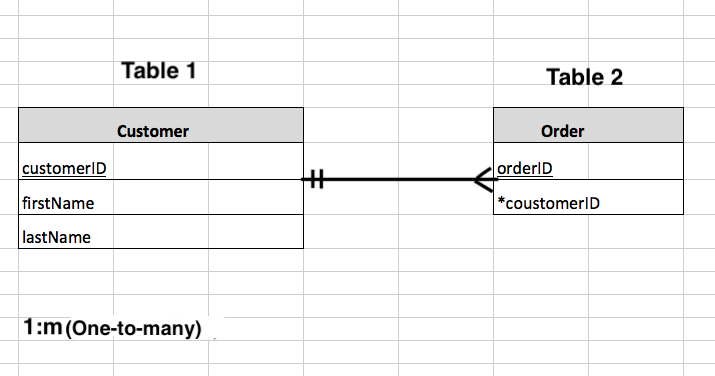
\includegraphics[width=115mm,scale=1]{figures/relational-db-relation.png}
    \caption{One-to-many relation between "Customer" and "Order"}
    \label{fig:relational-db-relation}
\end{figure}

SQL also offers a data manipulation language(DML) \cite{sql-components}.
The DML allows for the insertion of, retrieval of, update of, and deletion of data \cite{sql-dml-options}.
Whenever a tuple is added, updated or removed the tuple must conform to the restraints set by the DDL.
The attempted action will be aborted should there be discrepancies between the constraint of the table or column and the data.
This ensures that the data in the table is accurate and reliable \cite{sql-constraints}.

In addition SQL:
\begin{itemize}
    \item Provides an organized structure as data is defined once, and items referencing the data does so using foreign keys \cite{upwork-sql-adv}.
    \item Reduces data redundancy due to the organized structure \cite{upwork-sql-adv}.
    \item Allows JOIN operations \cite{upwork-sql-adv}.
    The operation allows two or more tables to be combined based on some shared attribute between them.
    The JOIN operation provides the ability to fetch specific data across tables that otherwise would prove cumbersome \cite{sql-joins}.
    \item Provides support for transactions.
    Transactions are essential in databases which require reliable data as they provide a framework for an all-or-nothing approach.
    This means the sequence of involved operations have to succeed in its entirety.
    The database will perform a rollback and raise an error should one of the operations fail \cite{sql-transactions}.
\end{itemize}

\subsection{NoSQL}
A NoSQL(Not only SQL) database provides data storage and data retrieval capabilities that is not modeled using a conventional RDBMS \cite{nosql-not-rdbms}.
Schema-less models are used instead of the traditional RDBMSs.
The most popular models include:
\begin{itemize}
    \item Key-value stores.
    Every item in the database is stored as an attribute name with a corresponding value \cite{mongodb-explains-nosql}.
    The key and value can be anything, and the key acts as a unique identifier for the value \cite{nosql-key-value}.
    \item Document databases.
    Document databases are an extension to key-value stores.
    Documents are structures which can contain many different key-pairs, and documents can even contain other documents.
    The documents can store data in different format, such as XML or JSON.
    Document databases are intended to store semi-sorted data \cite{nosql-document-sort}.
    \item Wide-column stores.
    The data in the database is stored in columns rather than the typical SQL rows.
    A given row can therefore have columns that other rows does not have.
    A wide-column store can be considered a two-dimensional key-value store \cite{infoworld-sql-vs-nosql}.
    \item Graph stores.
    The data in the database is represented as a graph.
    Their intended use is to traverse and navigate relationships.
    These databases use nodes to represent items in the database, and an edge between two nodes represents a relationship between the two items \cite{nosql-graph}.
\end{itemize}

NoSQL is advantageous because it:
\begin{itemize}
    \item Allows for semi-structured or unstructured data in the database.
    This flexible design allows the database to handle changes in structure more easily, and also allows the database to scale with ease \cite{mongodb-adv-nosql}.
    \item Allows for data to be inserted without a schema \cite{omkarsoft-adv-nosql}.
    This is beneficial should data be expected to change during the development of the project.
    \item Scales horizontally rather than vertically \cite{mongodb-adv-nosql}.
    Scaling horizontally allows partitions of data to be scatted across several pieces of hardware in order to store the data in the database.
    By contrast, scaling vertically means replacing already-existing hardware with more powerful hardware \cite{technopedia-nosql-scale}.
\end{itemize}

\subsection{Why SQL is the selected database system}
The assignment provider believes a SQL database system is more suited for the project than that of a NoSQL database system.
The equipment provided at MakerSpace is limited in quantity - as such the data to be stored in the database is also small in scale.
Due to the limited data the schema is simple to define, and as the requirements for the project are unlikely to change at a structural level the flexibility a NoSQL schema provides is not necessary.
The database is also likely to be stored in a limited number of locations and as such the distributed scaling capabilities a NoSQL database system offers is not particularly beneficial.
Overall the benefits provided by a NoSQL database system are not well suited for the project nor the scope of it which makes the SQL database system the preferable choice due to its organized structure, its relational properties and its support for JOIN operations.

\subsection{MariaDB as software}
MariaDB is the assignment providers database management system of choice.
MariaDB is one of the most popular\cite{mariadb-foundation-about} open source relational database management systems in the world \cite{mariadb-about}.
It is a fork of the also popular relational database management system MySQL\cite{mysql-about}.
MariaDB is made by the original developers behind MySQL \cite{mariadb-foundation-about} and it has a large list of sponsors providing financial support including Microsoft and IBM \cite{mariadb-sponsors}.
MariaDB is based on the SQL database system \cite{mariadb-about-searchdatamanagement}.

MariaDB has several notable features.
It is able to handle small and large data alike making it highly scalable, and it allows for rapid access to the data.
MariaDB releases stable releases, and each new release brings speed and stability improvements in addition to new features.
Additionally it places a high value of security - all data is encrypted by default and whenever critical security issues arise a new release is prepared \cite{mariadb-about}.
Lastly MariaDB offers a Node.js connector allowing applications developed on Node.js to connect to MariaDB \cite{mariadb-node-connector}.

\todo{Ikkje bruk several - ver konkret.}
\section{Frontend technology selection} 

The assignment provider wanted a full JavaScript technology stack and as such there were several technologies that could have been chosen for the frontend development. There are several JavaScript frontend frameworks and libraries freely available and as such this was not a big limitation \cite{JavaScript_libraries}.

\subsection{Vue.js}
Vue.js is a progressive JavaScript framework created by Evan You. Being a progressive framework means the user is able to select what features to include, instead of selecting which features not to include. By having a progressive framework you can make a web application only include the minimum of necessary components to work. This is one of the major features of the framework Vue.js. The core library of Vue.js is heavily focused on the view layer only, and is easy to integrate in already existing projects or other libraries \cite{what_is_Vue}. 

Easy Learning Curve
    All you need to know is html and ES5 JavaScript

Vue components

Native Reactivity

Template

Component scoped css

\subsection{React}
JSX



\subsection{Angular}
TypeScript

Learning Curve steep

\subsection{Our solution}
The group decided to recommend using Vue.js because of three major factors; the size of the framework, live updating in the browser and the low learning curve it has. Vue.js is comparably smaller than many of the other big JavaScript frameworks. It is roughly 58.8 kB in size. Since the framework is so small it will help with the loading speed of the web application \cite{vue-size}. 

The second major point for choosing Vue.js was the reactivity of Vue. With the reactivity of Vue.js you could update individual components based off of which data had been updated in the database. In Vue.js each component has getters and setters that enables Vue to track each component for when it's been accessed or modified. Each component also has a watcher instance that will be notified when that components setter is triggered. When this happens the watcher will notify Vue to run the component render function on that component again. With this feature there will be no need to update the whole site to show an update in the database \cite{vue-reactivity}. 

\begin{figure}[h]
    \centering
    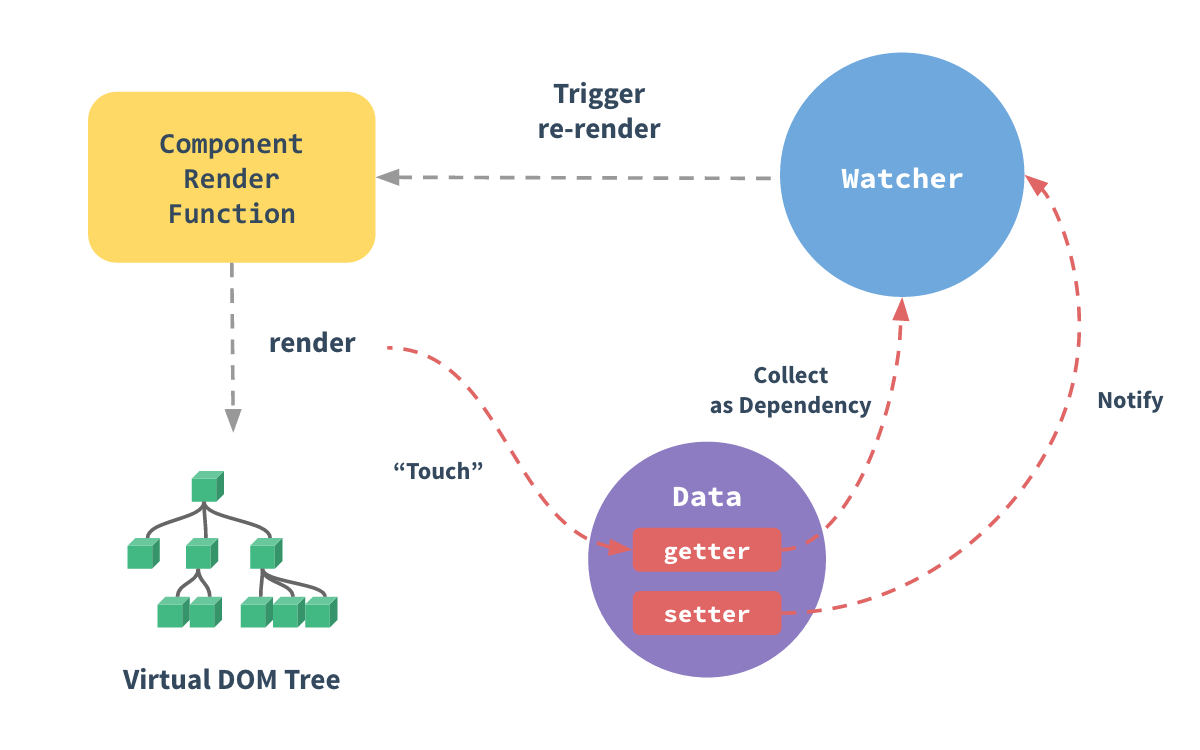
\includegraphics[width=115mm,scale=1]{figures/reactivity.png}
    \caption{Reactivity in Vue.js}
    \label{fig:vue_reactivity}
\end{figure}

The last major point for the group was the low learning curve of Vue.js. With this learning curve it means that the easier parts of Vue.js is easier to learn, but the more complicated components can be harder. This is perfect for the groups project since all the group members are new to Vue.js and can get faster into the programming.

The assignment provider agreed with the groups recommendation of Vue.js and allowed to project to be built using Vue.js

\section{Style sheet}
A style sheet is a file that is used in word processing and to define layout style of a document\cite{Style_sheet}.
For Microsoft Word as an example, the style sheets is known as a template\cite{Style_sheet}.
A style sheet contains specifications of a document layout\cite{Style_sheet}. 
The specifications is what page size, margins, fonts and font sizes is going to be set on the document\cite{Style_sheet}.
The group will not dive into what template is going to be used for Microsoft Word, but rather what style sheet is going to be used when developing a web system. Below it can be read what style sheet that will be used in the project and also what units and selectors that will be used. 

\subsection{CSS} \todo{Skriv om SVG og XML + referer til bildet. Gå til Waterfall og referer til bildet der også}
Cascading style sheet or "CSS" is used in any web application one way or another\cite{CSS_Introduction}. %and it will be used in the MakerSpace Management System web application.
CSS provides the visual aesthetics for the webpage by taking HyperText Markup Language (HTML), Scalable Vector Graphics (SVG) or Extensible Markup Language (XML) and converting it into a presentable form\cite{What_is_CSS}. This is done by web browsers applying CSS rules to an HTML document to affect how it is displayed. SVG is a text based open web standard designed to work with CSS and Document Object Model (DOM). It is an XML based text mark up language for two dimensional vector graphics\cite{SVG_definition}. SVG works by defining its data in XML text files and can be searched, indexed, scripted and compressed\cite{SVG_functions}. XML is a text-based format for representing and sharing structured information\cite{What_is_XML}. Figure 2.4 is a simple example of a CSS rule. The "p" stands for "paragraph" and within the brackets we declare that the color(property) is "red"(property value). The result would be the paragraphs text color will be red.
\begin{figure}[h]
    \centering
    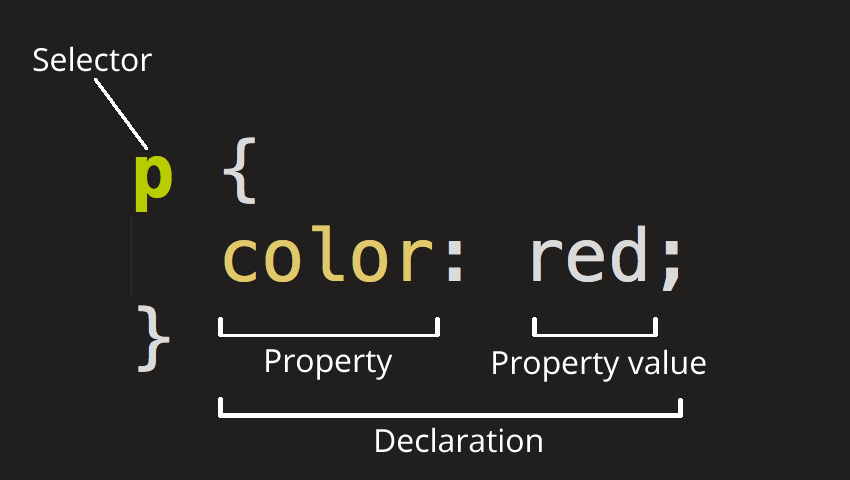
\includegraphics[width=80mm]{figures/css-declaration-small.png}
    \caption{CSS rule}
    \label{fig:Css rule example}
\end{figure}
When a webpage is being displayed, what is actually happening is the browser combining the document (HTML) with the CSS information\cite{CSS_and_DOM}. This process happens in two stages, where stage one converts the HTML and CSS into DOM\cite{What_is_DOM}. In figure 2.5 the stages of combining HTML and CSS is shown. The DOM is the PC's memory where the content of the HTML and CSS is combined. Stage two is the browser showing the content of the DOM where the webpage is displayed in all its glory with CSS applied to the HTML.

\begin{figure}[h]
    \centering
    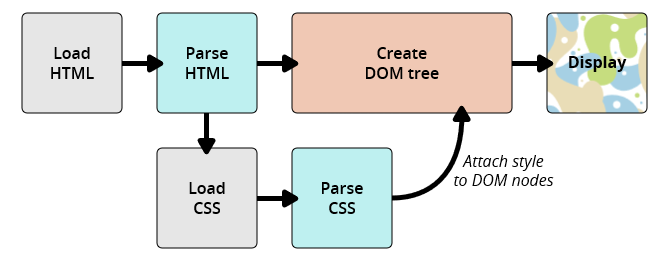
\includegraphics[width=130mm]{figures/DOM.png}
    \caption{HTML and CSS into DOM}
    \label{fig:DOM}
\end{figure}
\clearpage
% bildet plaseres ikke der den skal!!

\subsection{SASS}
SASS or "Syntactically Awesome Style Sheets" is a preprocessor scripting language that is compatible with all versions of CSS \cite{Sass_1}. 
With that it means it is possible to use any available CSS libraries that exists. Sass consists of two different syntaxes, the orginal syntas that they call "the indented syntax" (SASS) and the other one that is a newer syntax called "SCSS" (Sassy CSS)\cite{Sass_2}. 
The first syntax is build like it have indentation to separate code blocks and newline characters to separate rules. The other syntax (SCSS) uses block formatting like in CSS. It uses braces to denote code blocks and semicolons to separate lines within a block. The syntax SASS and SCSS files are also given the extensions .sass and .scss \cite{Sass_2}. 
Below it shows the syntax differences between SASS and SCSS. 

\begin{figure}[h]
    \centering
     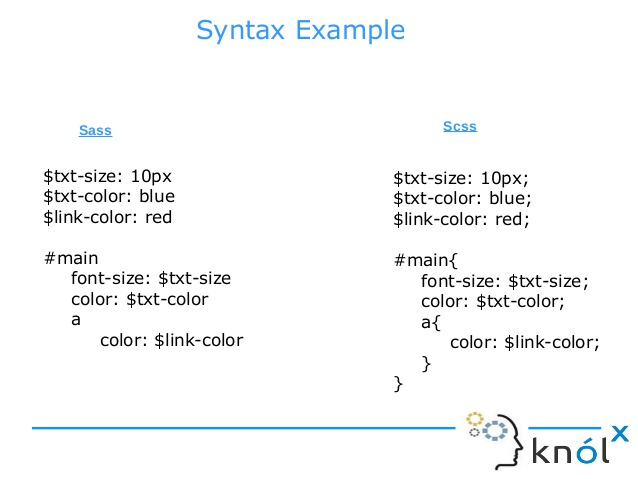
\includegraphics[width=115mm,scale=1]{figures/sass_and_scss.png}
    \caption{SASS and SCSS syntax}
    \label{fig:Sass}
\end{figure}


what SASS can offer in which 
CSS alone can't, is that Sass can use variables, mathematical operations, loops, functions, imports, and other  functionalities that make writing CSS much more powerful \cite{Sass_3}. 
This can be good when working with a large and complex sites.

One of the greatest benefits 
by using SASS is as mentioned the ability to use variables. A variable allows to store a value or a set of values, and to reuse these variables through the SASS files as many times as desired \cite{Sass_3}. 
This make the developers job a lot easier as for example if one want to use a color, instead of remember the color code, it can be stored as a describing variable that can be used everywhere in the project.

\subsection{Conclusion}
The project group in addition of agreement from the assignment provider have found out that it will be used SASS for this project. SASS is as mentioned compatible with all versions of CSS, only with more functionality. By choosing SASS the group think it will be taking benefits from its functionality that SASS offers. For this project it will only be developed a simple prototype, but for 
those who will take over the project, it will be nice that they have the opportunity to use this kind of functionality that SASS offers when the project get bigger and more complex. This since the group also have to think about that other can further develop the system.

\subsection{Units}
As the SASS was selected as a style sheet, the group needed also to find out what units to use with the style sheet. Units is what that can be used together with properties. Properties can for an example be length, where it can be used width or margin to set the length of an element \cite{Units_1}. 
Units is what defines the actual length of the element.

It exist two different length units, absolute and relative units \cite{Units_1}.
\begin{enumerate}
  \item \textbf{Absolute units:} The absolute length units are fixed, that means that a length will appear as exactly that size. This can be good when the output medium is known, such as for print layout. On the other hand, absolute length units should not be used on screens, because screens sizes vary so much. 
  
  Some of the units that exists is: \textbf{cm} (centimeters), \textbf{mm} (millimeters) and \textbf{in} (inches).
  \item \textbf{Relative units:} Relative length units is specifying a length that is relative to another length property. Relative length units will scale better between different rendering mediums. In other hand, this is good when working with different screen size, and is much greater to use when one will adjust the SASS to several platforms as mobile, different PC screens and tablets. 
  
  Some of the units that exist is: \textbf{em} (relative to the font-size of the element), \textbf{rem} (relative to font-size of the root element) and \textbf{\%} (relative to the parent element).
\end{enumerate}

As that the group will be working with different screens and platforms and also want it to scale great, it will be relative units that is going to be used for the project. The assignment provider also agrees that this is the best solution.

\subsection{Class and id selectors}
The group will in this project use what called selectors. Selectors are used to find/or select a HTML elements based on their element name as id, class, element name etc \cite{selectors}. 
It will mostly be used id and class names.
\begin{itemize}
  \item \textbf{Id selector:}
The id selector uses a id attribute for a HTML element to select that specific element.
The id of an element need to be unique in 
each single page, with that it means that the id selector is used to select one unique element. To select a element with a id name, it needs to be written a hash (\#) character followed by the id name that has been set \cite{selectors}. 
  \item \textbf{Class selector:}
The class selector works a bit like id selectors. It is supposed to help with choosing a specific element by a name. The differences between id and class selectors, is that class selectors do not need to be unique. It can be several similar names defined in the same files. The good use of this is when there are several elements that need the same changes (for example if there are buttons that needs the same style), it can then be done with defining those elements with same class name, and by setting a specify a style to that class will make all the changes appear for all elements that have that same class name \cite{selectors}.

To select a element with a class name, it needs to be written a period (.) character followed by the name of the class.
\end{itemize}




\section{Backend technology selection}
\todo{en måte: alternativ valg +/- valget}
For the backend technology there are several technologies that could be used. The group had discussed what backend technology to use, and asked the assignment provider to choose. A full JavaScript technology stack was chosen and some of the major backend technologies have been ruled out. Such as Pythons Django, PHP or Javas Spring backend framework. 

JavaScript will be used for the backend, Node.js will be used as the server to create and handle the backend operations needed in the application. Node.js is a JavaScript run-time environment that can run JavaScript code outside of the browser using the V8 JavaScript engine. Node.js runs on a single thread and is able to do this because of the Event Loop. When a request gets sent to Node from the application it will be added to the event queue before being picked up by the Event Loop. The Event Loop will take these requests and send them to the system that Node runs on. Here each request will be sent to different threads and be completed. When the task in done a callback function in the request is activated and the feedback is sent directly back to the application. The reason this event loop is so efficient at handling requests is because it runs asynchronous. So when it receives a request and sends off a callback function for that request. It doesn't need to wait for that callback function to return something before it handles a new request \cite{Node-event-loop}.

\begin{figure}[h]
    \centering
    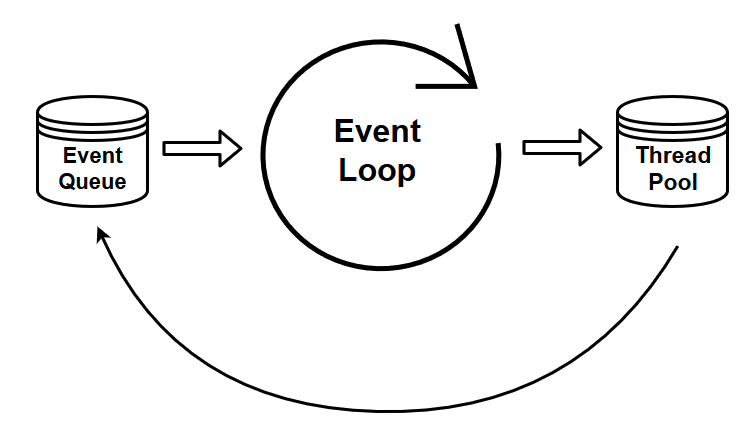
\includegraphics[width=100mm,scale=1]{figures/event_loop.png}
    \caption{Event loop in Node.js}
    \label{fig:Node_Event_Loop}
\end{figure}

\section{Connecting the frontend and the backend}
The frontend needs to be able to connect to the backend to create, read, update or delete resources.
The connection protocol selected is HTTP(Hypertext Transfer Protocol) and HTTPS(Hypertext Transfer Protocol Secure).

\subsection{HTTP and HTTPS}
HTTP is a protocol designed for communication between distributed systems \cite{mozilla_what_is_http}.
The flow of the protocol looks like this \cite{mozilla_http_flow}:
\begin{enumerate}
    \item The client sends an HTTP request to the target host.
    \item The host receives the HTTP request.
    \item The host processes the HTTP request.
    \item The host sends an HTTP response to the client.
    \item The client receives the HTTP response.
\end{enumerate}

HTTPS is an extension of HTTP \cite{http_vs_https}.
HTTP transmits data in plain text, and as such the protocol is considered insecure as anyone listening or intercepting the traffic can read the data transmitted \cite{http_vs_https}.
HTTPS on the other hand encrypts the data before transmitting it to an external host \cite{https_explained}.
This ensures anyone listening or intercepting the traffic is unable to read the data.
All data can thus pass freely and securely between the two hosts communicating with one another \cite{http_vs_https}.

HTTP/HTTPS lays the foundation for any data exchange \cite{mozilla_http_overview} on the modern web \cite{tutsplus_what_is_http} which makes the protocols the ideal protocols for communication between the frontend and the backend for the project.

\subsection{HTTP request methods}
HTTP request methods indicate the desired action to be performed on the given resource.
There are several HTTP request methods \cite{mozilla_http_status_methods_list} however the application is likely to use some of the following:
\begin{itemize}
    \item GET indicates the client wishes to retrieve the data for the resource identified with the resource identifier provided in the HTTP request, or the client indicates - in the absence of such an identifier - it wishes to retrieve the data for all resources \cite{mozilla_http_status_methods_list}.
    \item POST indicates the client wishes to create a new resource with the provided data in the HTTP request \cite{mozilla_http_status_methods_list}.
    \item PUT indicates the client wishes to update the resource identified with the resource identifier provided in the HTTP request \cite{mozilla_http_status_methods_list}.
    \item DELETE indicates the client wishes to delete the resource identified with the resource indentifier provided in the HTTP request \cite{mozilla_http_status_methods_list}.
\end{itemize}

\subsection{HTTP status codes}
HTTP status codes are responses made by the server in response to a request made by the client indicating either success or failure of the request \cite{http_vs_https}.
All HTTP status codes are separated into the following categories \cite{mozilla_http}:
\begin{itemize}
    \item 1xx represents informational state; The request was received and understood but the server is still processing the request.
    \item 2xx represents successful state; The request was successfully received, understood and fulfilled.
    \item 3xx represents a state of redirection; The client must take further action to complete the initial HTTP request.
    \item 4xx represents client error; The request is invalid in some way and the initial request was therefore not fulfilled.
    \item 5xx represents server error: The server either failed to fulfill a seemingly valid request, refused to carry it out, or is otherwise incapable of carrying it out.
\end{itemize}

There are many HTTP status codes \cite{http_status_codes_list}.
To name a few the application is likely to use:
\begin{itemize}
    \item 200(OK) indicates the request succeeded \cite{mozilla_http_status_codes_success}.
    \item 201(Created) indicates the request succeeded and a new resource was created as a result of it \cite{mozilla_http_status_codes_success}.
    \item 400(Bad Request) indicates the server cannot or will not process the request due to errors believed to be produced by the client \cite{mozilla_http_status_codes_client_error}.
    \item 401(Unauthorized) indicates the client is not authenticated while attempting to perform an action which requires the client to be authenticated \cite{mozilla_http_status_codes_client_error}.
    \item 403(Forbidden) indicates the client is attempting to perform an action it is unauthorized to perform \cite{mozilla_http_status_codes_client_error}.
    \item 404(Not Found) indicates the request requested a resource which does not exist \cite{mozilla_http_status_codes_client_error}.
    \item 409(Conflict) indicates the request could not be processed because the request contained a resource in conflict with another resource \cite{mozilla_http_status_codes_client_error}.
    \item 500(Internal Server Error) indicates the server encountered an unexpected condition which it was unable to resolve \cite{mozilla_http_status_codes_server_error}.
\end{itemize}

\subsection{JSON}

\section{Git and GitHub}